\documentclass[]{article}
\newcommand{\FileDepth}{../..}
\input{\FileDepth/Formats/AssignmentBasics.tex}
\usepackage{cancel}%This is special for Activities 4 and 5.
%opening
\newcommand{\SecType}{X}
\newcommand{\Week}{X}
\title{Toy Rocket Launch}
\author{Benjamin Bauml}
\date{Winter 2025}
\pagestyle{fancy}
\rhead{PH 221}
\chead{Winter 2025}
\lhead{Week \Week}

% For Assignment, leave Purpose as 1. For Worksheet, set to 2. For Student Solution, set to 3. For Teacher Solution, set to 4.
% If you want keep the pieces from being called manually, set DefOnly to 0.
\newcommand{\Purpose}{4}
\newcommand{\DefOnly}{1}

% Version 2024-04-27
% Changes
% 2024-02-21 Added xstring package to enable smooth implementation of new \ModePage command.
% 2024-04-27 Set up to split activities and formatting aspects into separate files. Removed dependence on xcomment. Added an automatic counter to number the activities in a problem set.
\usepackage{tcolorbox}
\usepackage{xstring}
% You will want the following four lines in your document (the last two uncommented):
% For Assignment, leave Purpose as 1. For Worksheet, set to 2. For Student Solution, set to 3. For Teacher Solution, set to 4.
% If you want keep the pieces from being called manually, set DefOnly to 0.
%\newcommand{\Purpose}{4}
%\newcommand{\DefOnly}{1}
\newcommand{\Exclusion}{0}
\newcommand{\PageTurn}{0}
\newcommand{\GrayProb}{0}
\newcommand{\Tipsy}{0}

% Assignment
\if\Purpose1
\renewcommand{\Exclusion}{1}
\fi
% Worksheet
\if\Purpose2
\renewcommand{\Exclusion}{1}
\renewcommand{\PageTurn}{1}
\fi
% Student Solution
\if\Purpose3
\renewcommand{\PageTurn}{1}
\renewcommand{\GrayProb}{1}
\fi
% Teaching Copy
\if\Purpose4
\renewcommand{\PageTurn}{1}
\renewcommand{\GrayProb}{1}
\renewcommand{\Tipsy}{1}
\fi

\def \NewQ {0}
\def \PForce {0}
\newcommand{\MaybePage}[1]{
	\def \PForce {#1}
	\if\PForce1
	\newpage
	\else
	\if\NewQ0
	\gdef \NewQ {\PageTurn}
	\else
	\newpage
	\fi
	\fi
}

\newcommand{\ModePage}[1]{
	\IfSubStr{#1}{\Purpose}{\newpage}{}
}

\newcounter{ActNumber}
\setcounter{ActNumber}{0}

\newcommand{\Problem}[4][0]{%The first argument is optional, and if it is set to 1, the \newpage will be forced. The second argument is the name of the activity, the third is the command the activity is stored as, and the fourth is the actual problem statement.
\newcommand{#3}{
\MaybePage{#1}
\addtocounter{ActNumber}{1}
\section*{\SecType\Week-\theActNumber: #2}
\if\GrayProb1
\begin{tcolorbox}[colback=lightgray,colframe=lightgray,sharp corners,boxsep=1pt,left=0pt,right=0pt,top=0pt,bottom=0pt,after skip=2pt]
\else
\begin{tcolorbox}[colback=white,colframe=white,sharp corners,boxsep=1pt,left=0pt,right=0pt,top=0pt,bottom=0pt,after skip=2pt]
\fi
#4
\end{tcolorbox}\noindent
}
\if\DefOnly0
\else
#3
\fi
}
	
\newcommand{\ProblemSub}[3][0]{%The first argument is optional, and if a string of numbers is entered into it, it will force a \newpage in any \Purpose that shows up in the string. For example, "13" would lead to the newpage being forced in modes 1 and 3. The second is the command the activity is stored as, and the third is the actual problem statement.
\newcommand{#2}{
\ModePage{#1}
\if\GrayProb1
\begin{tcolorbox}[colback=lightgray,colframe=lightgray,sharp corners,boxsep=1pt,left=0pt,right=0pt,top=0pt,bottom=0pt,after skip=2pt]
\else
\begin{tcolorbox}[colback=white,colframe=white,sharp corners,boxsep=1pt,left=0pt,right=0pt,top=0pt,bottom=0pt,after skip=2pt]
\fi
#3
\end{tcolorbox}\noindent
}
\if\DefOnly0
\else
#2
\fi
}
		
\newcommand{\Solution}[2]{%The first argument is the command the solution is stored as, and the second is the actual solution.
\newcommand{#1}{
\if\Exclusion0
#2
\fi
}
\if\DefOnly0
\else
#1
\fi
}
		
\newcommand{\ProblemFig}[2]{%The first argument is the command the figure is stored as, and the second is the actual figure.
\newcommand{#1}{
\begin{figure}[h]
#2
\end{figure}
}
\if\DefOnly0
\else
#1
\fi
}
		
\newcommand{\TeachingTips}[1]{
\if\Tipsy1
\begin{tcolorbox}[colback=lightgray,colframe=black]
#1
\end{tcolorbox}
\fi
}

%\newcommand{\FBDaxes}[4][2]{
	\begin{scope}[shift={(#2)},rotate=#3]
		% x-axis
		\draw[thick,->] (-#1,0) -- (#1,0);
		\node[anchor=west] at (#1,0) {$x$};
		% y-axis
		\draw[thick,->] (0,-#1) -- (0,#1);
		\node[anchor=south] at (0,#1) {$y$};
		\coordinate (#4) at (0,0);
	\end{scope}
}
\newcommand{\FBDvectorMA}[4]{
	\begin{scope}[shift={(#1)}]
		\coordinate (#4tip) at ({#2*cos(#3)},{#2*sin(#3)});
		\draw[ultra thick,blue,->] (#1) -- (#4tip);
	\end{scope}
}
\newcommand{\FBDvectorXY}[3]{
	\begin{scope}[shift={(#1)}]
		\coordinate (#3tip) at (#2);
		\draw[ultra thick,blue,->] (0,0) -- (#3tip);
	\end{scope}
}
\newcommand{\FBDdot}[1]{
	\filldraw[black] (#1) circle (3pt);
}
\newcommand{\FBDbox}[5][1]{
	\begin{scope}[shift={(#2)},rotate=#3]
		\filldraw[color=black,fill=white,thick] ({-#1/2},{#1/2}) -- ({-#1/2},{-#1/2}) -- ({#1/2},{-#1/2}) -- ({#1/2},{#1/2}) -- cycle;
		% Left side coordinates
		\coordinate (#4ltq) at ({-#1/2},{#1/4});
		\coordinate (#4lcent) at ({-#1/2},0);
		\coordinate (#4lbq) at ({-#1/2},{-#1/4});
		% right side coordinates
		\coordinate (#4rtq) at ({#1/2},{#1/4});
		\coordinate (#4rcent) at ({#1/2},0);
		\coordinate (#4rbq) at ({#1/2},{-#1/4});
		% top coordinates
		\coordinate (#4tlq) at ({-#1/4},{#1/2});
		\coordinate (#4tcent) at (0,{#1/2});
		\coordinate (#4trq) at ({#1/4},{#1/2});
		% bottom coordinates
		\coordinate (#4blq) at ({-#1/4},{-#1/2});
		\coordinate (#4bcent) at (0,{-#1/2});
		\coordinate (#4brq) at ({#1/4},{-#1/2});
		% corners
		\coordinate (#4tl) at ({-#1/2},{#1/2});
		\coordinate (#4tr) at ({#1/2},{#1/2});
		\coordinate (#4bl) at ({-#1/2},{-#1/2});
		\coordinate (#4br) at ({#1/2},{-#1/2});
		\node at (0,0) {#5};
	\end{scope}
}

\begin{document}
\maketitle
\begin{center}
	This activity is Problem 22 of Chapter 2 from the \textit{Student Workbook} for \textit{Physics for Scientists and Engineers}.
\end{center}

\Problem{Toy Rocket Launch}{\ToyRocket}{
A toy rocket is launched straight up with constant acceleration $ a $. It runs out of fuel at time $ t $.
}
\ProblemSub{\ToyRocketA}{
(a) Is the rocket at its maximum height the instant it runs out of fuel? Explain briefly.
}
\Solution{\ToyRocketASol}{
No. It has been gaining speed since it launched, and now it still has upward velocity to carry it further.
}
\ProblemSub{\ToyRocketB}{
(b) What assumptions would you make in order to solve this problem?
}
\Solution{\ToyRocketBSol}{
First, we will be modeling the rocket as a point mass for simplicity. We are given the assumption that the rocket is launched perfectly straight up, so we don't have to worry about horizontal motion and may leave the problem completely one-dimensional. We should also assume that the rocket is near the Earth's surface (thus gravity does not change appreciably with elevation). We should ignore air resistance, which further helps us to assume that the acceleration of the object is constant as it falls (after the fuel runs out).
}
\ProblemSub{\ToyRocketC}{
(c) What is the name of motion under the influence of only gravity? How would you write the vector for acceleration due to gravity?
}
\Solution{\ToyRocketCSol}{
Motion under the influence of only gravity is called \textit{free-fall} (even if the object is moving upward during the motion; it does not need to be going down to be in free-fall).

Assuming that $\hat{y}$ points upward (a common and reasonable choice of coordinate system), then the vector for acceleration due to gravity would be $\vec{a}=-g\hat{y}$. Note that the negative sign comes from our coordinate system; the constant $g\approx9.8$ m/s is a positive quantity.
}
\ProblemSub[34]{\ToyRocketD}{
(d) Draw a motion diagram for this problem. You should have three identified points in the motion: launch, out of fuel, maximum height. We'll call these points 1, 2, and 3 to have consistent definitions.
\begin{itemize}
	\item Using subscripts, define quantities: $ y $, $ v_{y} $, and $ t $ at each of the three points, 
	\item Describe the acceleration $ a_{1} $ during the interval from point 1 to point 2, and acceleration $ a_{2} $ during the interval from point 2 to point 3.
	\item Identify each quantity as Unknown or Known:
	\begin{itemize}
		\item Was it given numerically? 
		\item Was it given symbolically? 
		\item Can we reason that it must be zero? 
		\item Be careful with signs!
	\end{itemize}
\end{itemize}
}
\Solution{\ToyRocketDSol}{
\begin{figure}[h]
	\centering
	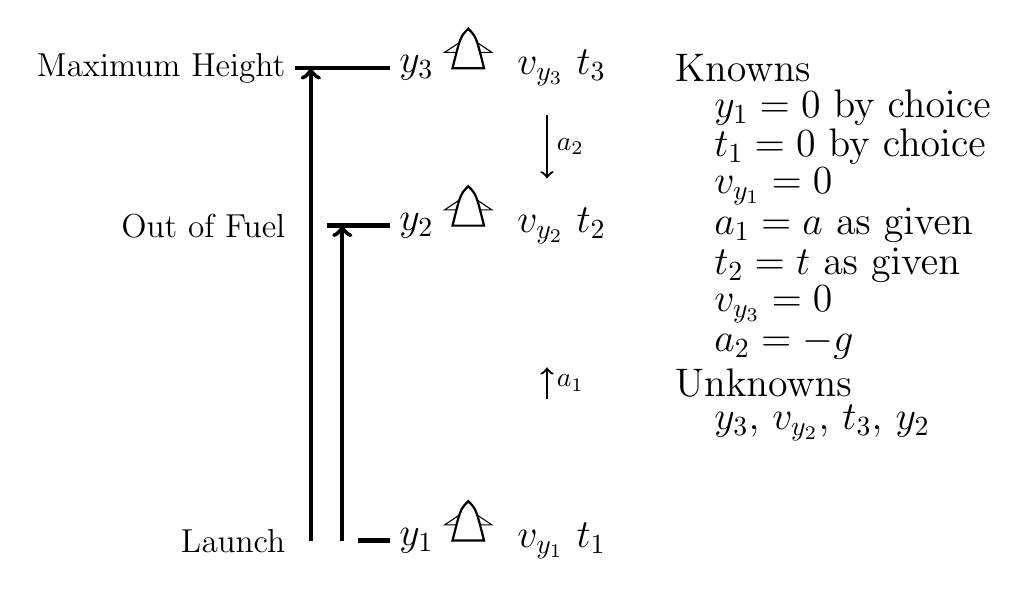
\begin{tikzpicture}
		\begin{scope}
			\draw (-0.3,0.2) -- (0.3,0.2) -- (0,0.4) -- cycle;
			\filldraw[white,draw=black,thick] (-0.2,0) -- (0.2,0) .. controls (0.1,0.4) .. (0,0.5) .. controls (-0.1,0.4) .. cycle;
			\node[anchor=west] at (0.5,0) {\Large$v_{y_{1}}$ $t_{1}$};
			\coordinate (y1) at (-1,0);
			\node[anchor=west] at (y1) {\Large$y_{1}$};
		\end{scope}
		\begin{scope}[shift={(0,4)}]
			\draw (-0.3,0.2) -- (0.3,0.2) -- (0,0.4) -- cycle;
			\filldraw[white,draw=black,thick] (-0.2,0) -- (0.2,0) .. controls (0.1,0.4) .. (0,0.5) .. controls (-0.1,0.4) .. cycle;
			\node[anchor=west] at (0.5,0) {\Large$v_{y_{2}}$ $t_{2}$};
			\coordinate (y2) at (-1,0);
			\node[anchor=west] at (y2) {\Large$y_{2}$};
		\end{scope}
		\begin{scope}[shift={(0,6)}]
			\draw (-0.3,0.2) -- (0.3,0.2) -- (0,0.4) -- cycle;
			\filldraw[white,draw=black,thick] (-0.2,0) -- (0.2,0) .. controls (0.1,0.4) .. (0,0.5) .. controls (-0.1,0.4) .. cycle;
			\node[anchor=west] at (0.5,0) {\Large$v_{y_{3}}$ $t_{3}$};
			\coordinate (y3) at (-1,0);
			\node[anchor=west] at (y3) {\Large$y_{3}$};
		\end{scope}
		\draw[ultra thick] (y1) -- (-1.4,0);
		\node[anchor=east] at (-2.2,0) {\large Launch};
		\draw[ultra thick] (y2) -- (-1.8,4);
		\draw[->,ultra thick] (-1.6,0) -- (-1.6,4);
		\node[anchor=east] at (-2.2,4) {\large Out of Fuel};
		\draw[ultra thick] (y3) -- (-2.2,6);
		\draw[->,ultra thick] (-2,0) -- (-2,6);
		\node[anchor=east] at (-2.2,6) {\large Maximum Height};
		\draw[->,thick] (1,5.4) -- (1,4.6);
		\node[anchor=west] at (1,5) {$a_{2}$};
		\draw[->,thick] (1,1.8) -- (1,2.2);
		\node[anchor=west] at (1,2) {$a_{1}$};
		\node[anchor=west] at (2.5,6) {\Large Knowns};
		\node[anchor=west] at (3,5.5) {\Large $y_{1} = 0$ by choice};
		\node[anchor=west] at (3,5) {\Large $t_{1} = 0$ by choice};
		\node[anchor=west] at (3,4.5) {\Large $v_{y_{1}} = 0$};
		\node[anchor=west] at (3,4) {\Large $a_{1} = a$ as given};
		\node[anchor=west] at (3,3.5) {\Large $t_{2} = t$ as given};
		\node[anchor=west] at (3,3) {\Large $v_{y_{3}} = 0$};
		\node[anchor=west] at (3,2.5) {\Large $a_{2} = -g$};
		\node[anchor=west] at (2.5,2) {\Large Unknowns};
		\node[anchor=west] at (3,1.5) {\Large $y_{3}$, $v_{y_{2}}$, $t_{3}$, $y_{2}$};
	\end{tikzpicture}
\end{figure}

We can set the starting height $y_{1}$ of the rocket to zero, and we can always choose to start counting time at the launch (therefore making $t_{1}=0$ s). The final velocity $v_{y_{3}}$ is zero by definition, as the rocket has no speed when it is at its maximum height. We can reason that the rocket starts from rest on the ground, so $v_{y_{1}}=0$ m/s. These are all of our numerical knowns.

Symbolically, we are given the out-of-fuel time, $t_{2} = t$, and the upward acceleration during the launch, $a_{2}=a$. Note that this is the overall acceleration, which accounts for both the downward pull of gravity and the stronger upward thrust of the rocket engine. We also know that $a_{2}=-g$, as the object is in free-fall after it runs out of fuel. It is negative, as the acceleration is downward and we are choosing up to be the positive direction.

That leaves $y_{2}$, $v_{y_{2}}$, $t_{3}$, and $y_{3}$ as unknowns.
}
\ProblemSub[34]{\ToyRocketE}{
(e) Draw qualitatively accurate graphs of the acceleration vs. time and the velocity vs. time.
}
\Solution{\ToyRocketESol}{
\begin{figure}[h]
	\centering
	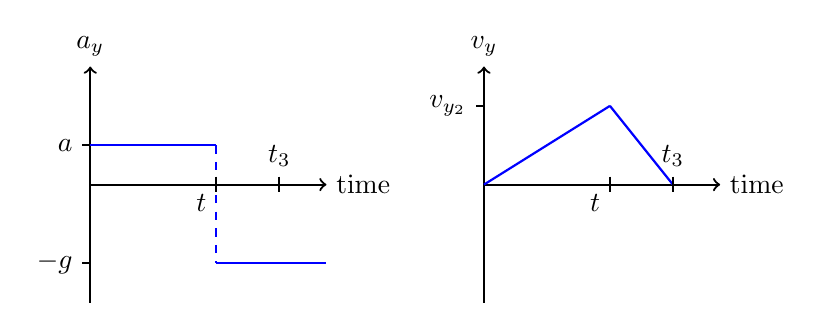
\begin{tikzpicture}
		\begin{scope}
			\draw[->,thick] (0,-1.5) -- (0,1.5);
			\node[anchor=south] at (0,1.5) {$a_{y}$};
			\coordinate (tend) at (3,0);
			\draw[->,thick] (0,0) -- (tend);
			\node[anchor=west] at (3,0) {time};
			\coordinate (aheight) at (0,0.5);
			\coordinate (gheight) at (0,-1);
			\coordinate (tlong) at (1.6,0);
			\coordinate (t3long) at (2.4,0);
			\begin{scope}[shift={(tlong)}]
				\coordinate (dtop) at (0,0.5);
				\coordinate (dbottom) at (0,-1);
				\draw[blue,thick,dashed] (dtop) -- (dbottom);
				\draw[thick] (0,0.1) -- (0,-0.1);
				\node[anchor=north east] at (0,0) {$t$};
			\end{scope}
			\draw[blue,thick] (aheight) -- (dtop);
			\draw[blue,thick] (dbottom) -- (tend |- gheight);
			\begin{scope}[shift={(aheight)}]
				\node[anchor=east] at (-0.1,0) {$a$};
				\draw[thick] (-0.1,0) -- (0,0);
			\end{scope}
			\begin{scope}[shift={(gheight)}]
				\node[anchor=east] at (-0.1,0) {$-g$};
				\draw[thick] (-0.1,0) -- (0,0);
			\end{scope}
			\begin{scope}[shift={(t3long)}]
				\draw[thick] (0,0.1) -- (0,-0.1);
				\node[anchor=south] at (0,0.1) {$t_{3}$};
			\end{scope}
		\end{scope}
		\begin{scope}[shift={(5,0)}]
			\draw[->,thick] (0,-1.5) -- (0,1.5);
			\node[anchor=south] at (0,1.5) {$v_{y}$};
			\coordinate (tend) at (3,0);
			\draw[->,thick] (0,0) -- (tend);
			\node[anchor=west] at (3,0) {time};
			\coordinate (aheight) at (0,1);
			\coordinate (gheight) at (0,-0.5);
			\coordinate (tlong) at (1.6,0);
			\coordinate (t3long) at (2.4,0);
			\begin{scope}[shift={(tlong)}]
				\coordinate (dtop) at (0,1);
				%\coordinate (dbottom) at (0,-0.5);
				%\draw[blue,thick,dashed] (dtop) -- (dbottom);
				\draw[thick] (0,0.1) -- (0,-0.1);
				\node[anchor=north east] at (0,0) {$t$};
			\end{scope}
			\draw[blue,thick] (0,0) -- (dtop);
			\draw[blue,thick] (dtop) -- (t3long);
			\begin{scope}[shift={(aheight)}]
				\node[anchor=east] at (-0.1,0) {$v_{y_{2}}$};
				\draw[thick] (-0.1,0) -- (0,0);
			\end{scope}
			\begin{scope}[shift={(t3long)}]
				\draw[thick] (0,0.1) -- (0,-0.1);
				\node[anchor=south] at (0,0.1) {$t_{3}$};
			\end{scope}
		\end{scope}
	\end{tikzpicture}
\end{figure}

Having constant acceleration means that the acceleration will consist of (piecewise) horizontal lines, and thus the velocity graph will be (piecewise) linear. Since the acceleration graph has a jump discontinuity at $t$, the velocity graph will have a corner (a place where the slopes do not match) at the same time.

These graphs were drawn to match the picture in part (d). If the rocket is assumed to cover less distance after the fuel runs out than before, then the area under the velocity graph must be smaller from $t$ to $t_{3}$ than from 0 to $t$. This also means that the slope is steeper from $t$ to $t_{3}$, so the acceleration due to gravity must have a greater magnitude than $a$.
}
\ProblemSub{\ToyRocketFGH}{
Suppose we want to know the maximum height of the rocket.
}
\ProblemSub{\ToyRocketF}{
(f) This is a two-part problem. Use your knowledge of calculus and motion to write \textit{kinematic equations} for the first part of the motion. Use the given (symbolic) values for $a_1$ and $t_2$ to determine---again symbolically---the two unknown quantities at point 2.
}
\Solution{\ToyRocketFSol}{
We know the time of flight, acceleration, and initial velocity, and we want to know $ v_{y_{2}} $, so the following equation is most relevant:
\[
v_{y_{2}}=v_{y_{1}}+a_{1}(t_{2}-t_{1}) = 0 + a(t-0) = at.
\]
We know the inital position and velocity, the acceleration, and the time of flight, and we want to find $ y_{2} $, so the following equation is most relevant:
\[
\begin{split}
	y_{2} & = y_{1}+v_{y_{1}}(t_{2}-t_{1})+\frac{1}{2}a_{1}(t_{2}-t_{1})^{2} \\
	& = 0+0+\frac{1}{2}a(t-0)^{2} = \frac{1}{2}at^{2}.
\end{split}
\]
}
\ProblemSub{\ToyRocketG}{
(g) Use your knowledge of calculus and motion to write similar \textit{kinematic equations} for the second interval of the motion. Just write the equations; don't solve it yet.
}
\Solution{\ToyRocketGSol}{
By this point, we know the acceleration (solely gravitational) and the final velocity $ v_{y_{3}} = 0 $, and we would know $ y_{2} $ and $ v_{y_{2}} $ if we solved the above equations. We want to know the maximum height $ y_{3} $, so it would make sense to take the equation
\[
\begin{split}
	y_{3} & = y_{2}+v_{y_{2}}(t_{3}-t_{2})+\frac{1}{2}a_{2}(t_{3}-t_{2})^{2} \\
	& = y_{2} + v_{y_{2}}(t_{3}-t) - \frac{1}{2}g(t_{3}-t)^{2}.
\end{split}
\]
However, we need $t_{3}$ to solve this, so we can bring in the kinematic equation for velocity:
\[
\begin{split}
	v_{y_{3}} & = v_{y_{2}} + a_{2}(t_{3}-t_{2}) \\
	0 & = v_{y_{2}} - g(t_{3}-t).
\end{split}
\]
I will go ahead and combine these equations now in order to eliminate $t_{3}$. If I replace $t_{3}-t$ in the first equation with $\frac{v_{y_{2}}}{g}$, I get
\[
y_{3} = y_{2} + \frac{v^{2}_{y_{2}}}{g} - \frac{v^{2}_{y_{2}}}{2g} = y_{2} + \frac{v^{2}_{y_{2}}}{2g}.
\]
If you happen to know the third kinematic equation,
\[
v_{f}^{2} = v_{i}^{2} + 2a\Delta y,
\]
then you can skip the step of substituting for time and just obtain the prior result directly.
}
\TeachingTips{
Students may not have seen the third equation in class, and may be interested in seeing the derivation. Start with
\[
v_{f} = v_{i} + a\Delta t,
\]
and square it to get
\[
v_{f}^{2} = v_{i}^{2} + 2v_{i}a\Delta t + a^{2} (\Delta t)^{2}.
\]
Now take
\[
\Delta y = v_{i}\Delta t + \frac{1}{2} a (\Delta t)^{2},
\]
and multiply it by $2a$ to get
\[
2a\Delta y = 2v_{i}a\Delta t + a^{2} (\Delta t)^{2}.
\]
This substitutes cleanly into the prior equation to give
\[
v_{f}^{2} = v_{i}^{2} + 2a\Delta y.
\]
}
\ProblemSub{\ToyRocketH}{
(h) Now, substitute the known information from previous parts of the question into your equations from part (g). Find $y_3$ in terms of quantities given in the problem and the constant $g$.
}
\Solution{\ToyRocketHSol}{
We begin with
\[
y_{3} = y_{2} + \frac{v^{2}_{y_{2}}}{2g}.
\]
We know that $ v_{y_{2}} = at $ and $ y_{2} = \frac{1}{2}at^{2} $, so we get
\[
y_{3} = \frac{1}{2} at^{2} + \frac{a^{2}t^{2}}{2g} = \frac{(ga+a^{2})t^{2}}{2g}.
\]
}
\end{document}